% arara: pdflatex
% arara: bibtex
% arara: pdflatex
% arara: pdflatex


% options:
% thesis=B bachelor's thesis
% thesis=M master's thesis
% czech thesis in Czech language
% english thesis in English language
% hidelinks remove colour boxes around hyperlinks

\documentclass[thesis=M,english]{template/FITthesis}[2019/12/23]

\usepackage[utf8]{inputenc} % LaTeX source encoded as UTF-8
% \usepackage[latin2]{inputenc} % LaTeX source encoded as ISO-8859-2
% \usepackage[cp1250]{inputenc} % LaTeX source encoded as Windows-1250

% \usepackage{subfig} %subfigures
% \usepackage{amsmath} %advanced maths
% \usepackage{amssymb} %additional math symbols

\usepackage{graphicx}
\usepackage{dirtree} %directory tree visualisation
\usepackage{pdfpages}
\usepackage{import}
% \usepackage{xevlna}

% % list of acronyms
\usepackage[acronym]{glossaries}
% \iflanguage{czech}{\renewcommand*{\acronymname}{Seznam pou{\v z}it{\' y}ch zkratek}}{}
\makeglossaries

% % % % % % % % % % % % % % % % % % % % % % % % % % % % % %
% EDIT THIS
% % % % % % % % % % % % % % % % % % % % % % % % % % % % % %

\department{Department of Software Engineering}
\title{Cross-platform mobile application for safer drone operations}
\authorGN{Jan} %author's given name/names
\authorFN{Mat{\v e}jka} %author's surname
\author{Jan Mat{\v e}jka} %author's name without academic degrees
\authorWithDegrees{Bc. Jan Mat{\v e}jka} %author's name with academic degrees
\supervisor{Ing. Luk{\' a}{\v s} Brchl}
\acknowledgements{I would like to thank my family, my girlfriend and friends for support while writing this thesis and all my studies.
I also would like to thank my supervisor Ing. Luk{\' a}{\v s} Brchl, for this chance to realize me in mobile application development.}

%----------------------------------------------------------------------------------------------------------------------------------------

\abstractEN{This master's thesis focuses on cross-platform mobile application development in the Flutter framework for safer drone operations.
This thesis contains a full application analysis, design, and implementation.
Its main functionality is the managing drones and identification devices attached to drones, showing restricted flight zones, and planning and watching drone flights.

The analysis emphasizes the analysis of the existing web platform and all infrastructure, which provides data to the client and third-party applications.
The design contains a description of the application structure and uses architecture patterns of the Flutter framework.
The implementation describes details about realization and contains detailed launch instructions in the development, test, and production environments.
In addition, it contains a description of the necessary configuration files.
These files differ across the various environments and have a security disposition.}

%----------------------------------------------------------------------------------------------------------------------------------------

\abstractCS{Tato diplomov{\' a} pr{\' a}ce se zab{\' y}v{\' a} v{\' y}vojem multiplatformn{\' i} mobiln{\' i} aplikace ve frameworku Flutter pro bezpe{\v c}n{\v e}j{\v s}{\' i} provoz dron{\r u}.
Pr{\' a}ce obsahuje kompletn{\' i} anal{\' y}zu, n{\' a}vrh a samotnou implementaci aplikace, jej{\' i}{\v z} hlavn{\' i} fukcionalitou je spr{\' a}va dron{\r u} a identifika{\v c}n{\' i}ch za{\v r}{\' i}zen{\' i} p{\v r}ipevn{\v e}n{\' y}ch k dron{\r u}m, zobrazov{\' a}n{\' i} zak{\' a}zan{\' y}ch z{\' o}n pro lety a pl{\' a}nov{\' a}n{\' i} a sledov{\' a}n{\' i} let{\r u} dron{\r u}.

V anal{\' y}ze je kladen d{\r u}raz na rozbor existuj{\' i}c{\' i} webov{\' e} platformy a cel{\' e} infrastruktury, kter{\' a} poskytuje data klientsk{\' y}m aplikac{\' i}m a aplikac{\' i}m t{\v r}et{\' i}ch stran.
N{\' a}vrh obsahuje popis struktury aplikace a pou{\v z}it{\' e} architektonick{\' e} vzory frameworku Flutter.
Implementace popisuje detaily o realizaci a obsahuje podrobn{\' y} n{\' a}vod pro spu{\v s}t{\v e}n{\' i} ve v{\' y}vojov{\' e}m, testovac{\' i}m a produk{\v c}n{\' i}m prost{\v r}ed{\' i}.
Z{\' a}rove{\v n} obsahuje popis d{\r u}le{\v z}it{\' y}ch konfigura{\v c}n{\' i}ch soubor{\r u}, kter{\' e} se li{\v s}{\' i} nap{\v r}{\' i}{\v c} r{\r u}zn{\' y}mi prost{\v r}ed{\' i}mi a maj{\' i} bezpe{\v c}nostn{\' i} charakter.}

%----------------------------------------------------------------------------------------------------------------------------------------

\placeForDeclarationOfAuthenticity{Prague}
\keywordsCS{Multiplatformn{\' i}, mobiln{\' i}, aplikace, dron, {\v r}{\' i}zen{\' i}, Flutter}
\keywordsEN{Cross-platform, mobile, application, drone, operation, Flutter}
\declarationOfAuthenticityOption{6} %select as appropriate, according to the desired license (integer 1-6)
% \website{http://site.example/thesis} %optional thesis URL


\begin{document}

\newacronym{amsl}{AMSL}{Above Mean Sea Level}
\newacronym{agl}{AGL}{Above Ground Level}
\newacronym{utm}{UTM}{Unmanned Traffic Management}
\newacronym{ctr}{CTR}{Control zone}
\newacronym{ead}{EAD}{European AIS Database}
\newacronym{laanc}{LAANC}{Low Altitude Authorization and Notification Capability}
\newacronym{api}{API}{Application Programming Interface}
\newacronym{sdk}{SDK}{Software Development Kit}
\newacronym{sms}{SMS}{Short Message Service}
\newacronym{caa}{CAA}{Civil Aviation Authority}
\newacronym{nats}{NATS}{National Air Traffic Services}
\newacronym{ais}{AIS}{Aeronautical Information Services}
\newacronym{bloc}{BLoC}{Business Logic Component}
\newacronym{cd}{CD}{Continuous Delivery}
\newacronym{ci}{CI}{Continuous Integration}
\newacronym{chmi}{CHMI}{Czech Hydrometeorological Institute}
\newacronym{di}{DI}{Dependency Injection}
\newacronym{geojson}{GeoJSON}{Geographical JSON}
\newacronym{gps}{GPS}{Global Positioning System}
\newacronym{hifi}{Hi-Fi}{High Fidelity}
\newacronym{http}{HTTP}{Hypertext Transfer Protocol}
\newacronym{icao}{ICAO}{International Civil Aviation Organization}
\newacronym{ioc}{IoC}{Inversion of Control}
\newacronym{iot}{IoT}{Internet of Things}
\newacronym{json}{JSON}{Java Script Object Notation}
\newacronym{jwt}{JWT}{JSON Web Token}
\newacronym{k8s}{K8s}{Kubernetes}
\newacronym{lofi}{Lo-Fi}{Low Fidelity}
\newacronym{mvc}{MVC}{Model-View-Controller}
\newacronym{mvpres}{MVP}{Model-View-Presenter}
\newacronym{mvprod}{MVP}{Most Value Product}
\newacronym{mvvm}{MVVM}{Model-View-ViewModel}
\newacronym{notam}{NOTAM}{Notice To Airmen}
\newacronym{poi}{POI}{Point of Interest}
\newacronym{svg}{SVG}{Scalable Vector Graphics}
\newacronym{uas}{UAS}{Unmanned aircraft systems}
\newacronym{ui}{UI}{User Interface}
\newacronym{ux}{UX}{User Experience}
\newacronym{url}{URL}{Uniform Resource Locator}
\newacronym{rsrp}{RSRP}{Reference Signal Receive Power}
\newacronym{nosql}{NoSQL}{Not only Structure Query Language}
\newacronym{gdpr}{GDPR}{General Data Protection Regulation}
\newacronym{apk}{APK}{Android Package}
\newacronym{ipa}{IPA}{iOS App Store Package}
\newacronym{css}{CSS}{Cascade Style Sheet}
\newacronym{html}{HTML}{HyperText Markup Language}
\newacronym{devops}{DevOps}{Development and Operations}
\newacronym{db}{dB}{Decibel}

% \newacronym{CVUT}{{\v C}VUT}{{\v C}esk{\' e} vysok{\' e} u{\v c}en{\' i} technick{\' e} v Praze}
% \newacronym{FIT}{FIT}{Fakulta informa{\v c}n{\' i}ch technologi{\' i}}


\setsecnumdepth{part}
\chapter{Introduction}\label{ch:introduction}
This thesis is focused on ...
Since 2017, RLP is solving a problem with managing of flight drone operations.
It is the reason why this thesis was established.

\section{Motivation}\label{sec:motivation}
TODO
Řízení leteckého provozu
Exponenciální trh
úspěchy Dronetagu v soutěžích, Hackathonech

\section{Objectives}\label{sec:objectives}
TODO
Mobile app distributable to stores

\section{Problem statement}\label{sec:problem-statement}
TODO
Drones problematics

\setsecnumdepth{all}
\chapter{Related projects}\label{ch:related-projects}

In the world TODO - describe using of drones in industry
Amazon using/usage/application

autonomous drones application

describe potential using

\section{Project in Dronetag s.r.o. company}\label{sec:project-in-dronetag-s.r.o.-company}
describe the complex concept how can common user can use it for (Dronetag Pro and Mini)


\chapter{Dronetag web infrastructure}\label{ch:dronetag-web-infrastructure}
This chapter describes all Dronetag web infrastructure and contains a detailed description of the web Dronetag platform.
It consists of the all technical stack that ensures data providing and processing.
We had to determine a convenient and reliable way of how to construct a useful architecture of infrastructure gradually.
It starts with an IoT module and frontend web client written in JavaScript, and it continues to implement WebSockets in Live Service implementation based on a Kubernetes cluster.
Current parts of the stack are the following:
\begin{itemize}
    \item Load Balancer - it ensures load balancing of received requests (It redirects the requests to an available node in cluster.),
    \item Backend - it ensures communication with Database storage of data and provides API endpoint to allow drone security operation,
    \item Frontend - it ensures managing and watching drones activity via a web browser,
    \item Private API endpoint - it ensures API endpoint to give into or get private data from Dronetag platform (It is a part of Backend.),
    \item Public API endpoint - it ensures API endpoint to give into or get public data from Dronetag platform (It is also a part of Backend.),
    \item Database Storage that ensures persistent storing of data and
    \item Live Service - it ensures quick providing of Live data from airspace by the given viewport.
\end{itemize}
%The components and their relations are shown on the infrastructure diagram~\ref{fig:infrastracture-diagram}.
I must note the stack is still involved anytime when we find out it is insufficient and the complexity of the all system is increasing.
In this case, we need to determine the cause and ensure load balancing among the parts of the stack.

\section{API separation}\label{sec:api-separation}
Due to security reasons, the web API divides itself into \textbf{Private} and \textbf{Public API} endpoints.
\textbf{Public API} is allowed to use by third-party consumers.
It can be anyone who would like using our data to ensure drone operation security.

In further determination, this infrastructure divides into the \textbf{Staging} and \textbf{Production} environment.
Staging is for development and testing purposes, and it usually runs on the same version as Production.
Production is like a mirror of Staging.
The difference is that the Production environment contains a previous version of the software that is released.

\section{Docker deployment}\label{sec:docker-deployment}
Every web application in the stack is deployed and managed by \textbf{Docker}.
It is the easiest way to develop and publish new version software.
However, in the beginning, let us clarify what the Docker is.
"Docker is a tool designed to make it easier to create, deploy, and run applications by using containers.
Containers allow a developer to package up an application with all of the parts it needs, such as libraries and other dependencies, and deploy it as one package.
By doing so, thanks to the container, the developer can rest assured that the application will run on any other Linux machine regardless of any customized settings that machine might have that could differ from the machine used for writing and testing the code."\cite{dockerDescription}

To read about what a Container is and how useful it can be for business and can see on their official websites~\cite{dockerContainer} or here~\cite{dockerDescription}.

Thanks to the \textbf{Docker Compose} tool, we can have separated parts of the infrastructure.
In the case of more significant changes, we have to change only one module, and others are without changes.
In a nutshell, we have more containers that each of them contains individual responsibility for their processing, and \textbf{Docker Compose} joins them together.
If I simplify it, \textbf{Docker Compose} works like a composer that takes separate containers, where each of them can launch different technologies and compose it together into one whole infrastructure.\cite{dockerCompose}


\section{Kubernetes}\label{sec:kubernetes}
"Kubernetes (K8s) is an open-source system for automating deployment, scaling, and management of containerized applications."~\cite{kubernetes}
It means that Kubernetes is a tool allowing a running cluster whose single nodes may be as Docker containers.
This approach ensures scalability, whereas the number of Docker containers can be huge and can be created and disposed of dynamically based on the loading.
The advantage of Kubernetes is that it can detect a note out of order and initialize and deploy a new one to stay the optimal performance

"It groups containers that make up an application into logical units for easy management and discovery.
Kubernetes builds upon \textit{15 years of experience of running production workloads at Google}~\cite{kubernetesArticle}, combined with best-of-breed ideas and practices from the community."~\cite{kubernetes}
Thanks to these experiences, Kubernetes is a fine grain, and the cluster hierarchy is merely maintainable.

"Though widespread interest in software containers is a relatively recent phenomenon, at Google we have been managing Linux containers at scale for more than ten years and built three different container-management systems in that time."~\cite{kubernetesArticle}
How you can see, the idea of containerization has a rich history.
However, there were Linux Containers before the Docker ones.
That is the reason why we use it for web development.
It is easy to scale, maintain, and able to deploy to Google Cloud Platform.

\section{Database model}\label{sec:database-model}
There is a database model figure in Dronetag backend.
The database model consists followings entities:
\begin{itemize}
    \item User,
    \item Aircraft,
    \item Device,
    \item Flight,
    \item Telemetry measurement,
    \item Organization,
    \item Fleet,
    \item Aircraft vendor,
    \item Aircraft model,
    \item Airspace zone,
    \item User preference and
    \item Organization preference.
\end{itemize}
A detailed diagram with relationships between entities is in the ERD Diagram of infrastructure in this picture.%\cite{fig:erd-diagram}

\subsection{User}\label{subsec:user}
This entity represents a user who signs up and logs in to the application.
...

All attributes are described like this:
\begin{itemize}
    \item id - represents the unique object identificator,
    \item email - represents ...
    \item full\_name - represents
    \item password\_hash - represents
    \item phone\_number - represents
    \item deleted - represents
    \item date\_created - represents
    \item data\_modified - represents
    \item last\_login - represents
    \item active - represents
    \item country - represents
\end{itemize}

\subsection{Aircraft}\label{subsec:aircraft}
This entity represents an aircraft that is connect with a Dronetag device.
...

All attributes are described like this:
\begin{itemize}
    \item id - represents the unique object identificator,
    \item name - represents an aircraft name for easier recognition in My aircraft list,
    \item uas\_operator\_id - represents a unique code identifying a pilot who registered this aircraft,
    \item weight - represents a weight of the aircraft,
    \item date\_created - represents a date when was an aircraft added,
    \item data\_modified - represents a date when was an aircraft changed,
    \item deleted - represents a date when was an aircraft deleted.
\end{itemize}

\subsection{Device}\label{subsec:device}
This entity represents a physical device that sends live information to the Dronetag platform.
...

All attributes are described like this:
\begin{itemize}
    \item id - represents the unique object identificator,
    \item serial\_number - represents ...
    \item name - represents
    \item type - represents
    \item comm\_id - represents
    \item date\_created - represents
    \item date\_modified - represents
    \item last\_battery - represents
    \item last\_rsrp - represents
    \item last\_message - represents
\end{itemize}

\subsection{Flight}\label{subsec:flight}
This entity represents it represents a flight that a user has created.
...

All attributes are described like this:
\begin{itemize}
    \item id - represents the unique object identificator,
    \item date\_planned\_start - represents ...
    \item date\_planned\_finish - represents ...
    \item date\_started - represents ...
    \item date\_finished - represents ...
    \item status - represents
    \item distance - represents
    \item duration - represents
    \item region\_geojson - represents
    \item max\_flight\_altitude - represents
    \item takeoff\_latitude - represents
    \item takeoff\_longitude - represents
    \item takeoff\_geo\_alt - represents
    \item takeoff\_pressure - represents
    \item public - represents
    \item date\_created - represents
    \item date\_modified - represents
    \item deleted - represents
\end{itemize}

\subsection{Telemetry measurement}\label{subsec:telemetry-measurement}
This entity represents a ...

All attributes are described like this:
\begin{itemize}
    \item time\_received - represents the unique object identificator,
    \item time - represents ...
    \item latitude - represents
    \item longitude - represents
    \item altitude - represents
    \item geo\_altitude - represents
    \item velocity\_x - represents
    \item velocity\_y - represents
    \item velocity\_z - represents
    \item gnss\_accuracy - represents
\end{itemize}

\subsection{Organization}\label{subsec:organization}
This entity represents a ...

All attributes are described like this:
\begin{itemize}
    \item id - represents the unique object identificator,
    \item name - represents ...
    \item description - represents
    \item date\_created - represents
    \item date\_modified - represents
    \item deleted - represents
\end{itemize}

\subsection{Fleet}\label{subsec:fleet}
This entity represents a ...

All attributes are described like this:
\begin{itemize}
    \item id - represents the unique object identificator,
    \item name - represents ...
    \item color - represents
    \item deleted - represents
    \item date\_created - represents
    \item date\_modified - represents
\end{itemize}

\subsection{Aircraft vendor}\label{subsec:aircraft-vendor}
This entity represents a ...

All attributes are described like this:
\begin{itemize}
    \item id - represents the unique object identificator,
    \item name - represents a vendor name.
\end{itemize}

\subsection{Aircraft model}\label{subsec:aircraft-model}
This entity represents a user who signs up and logs in to the application.
...

All attributes are described like this:
\begin{itemize}
    \item id - represents the unique object identificator,
    \item name - represents ...
    \item weight - represents
    \item vendor\_id - represents a relationship to a Vendor.
\end{itemize}

\subsection{Airspace zone}\label{subsec:airspace-zone}
This entity represents a ...

All attributes are described like this:
\begin{itemize}
    \item id - represents the unique object identificator,
    \item name - represents ...
    \item country - represents
    \item region\_geojson - represents
    \item date\_created - represents
    \item date\_modified - represents
\end{itemize}

\subsection{User preference}\label{subsec:user-preference}
This entity represents a ...

All attributes are described like this:
\begin{itemize}
    \item property - represents ...
    \item value - represents ...
    \item date\_modified - represents
\end{itemize}

\subsection{Organization preference}\label{subsec:organization-preference}
This entity represents a user who signs up and logs in to the application.
...

All attributes are described like this:
\begin{itemize}
    \item property - represents the unique object identificator,
    \item value - represents ...
    \item date\_modified - represents
\end{itemize}

\begin{figure}
    \centering
    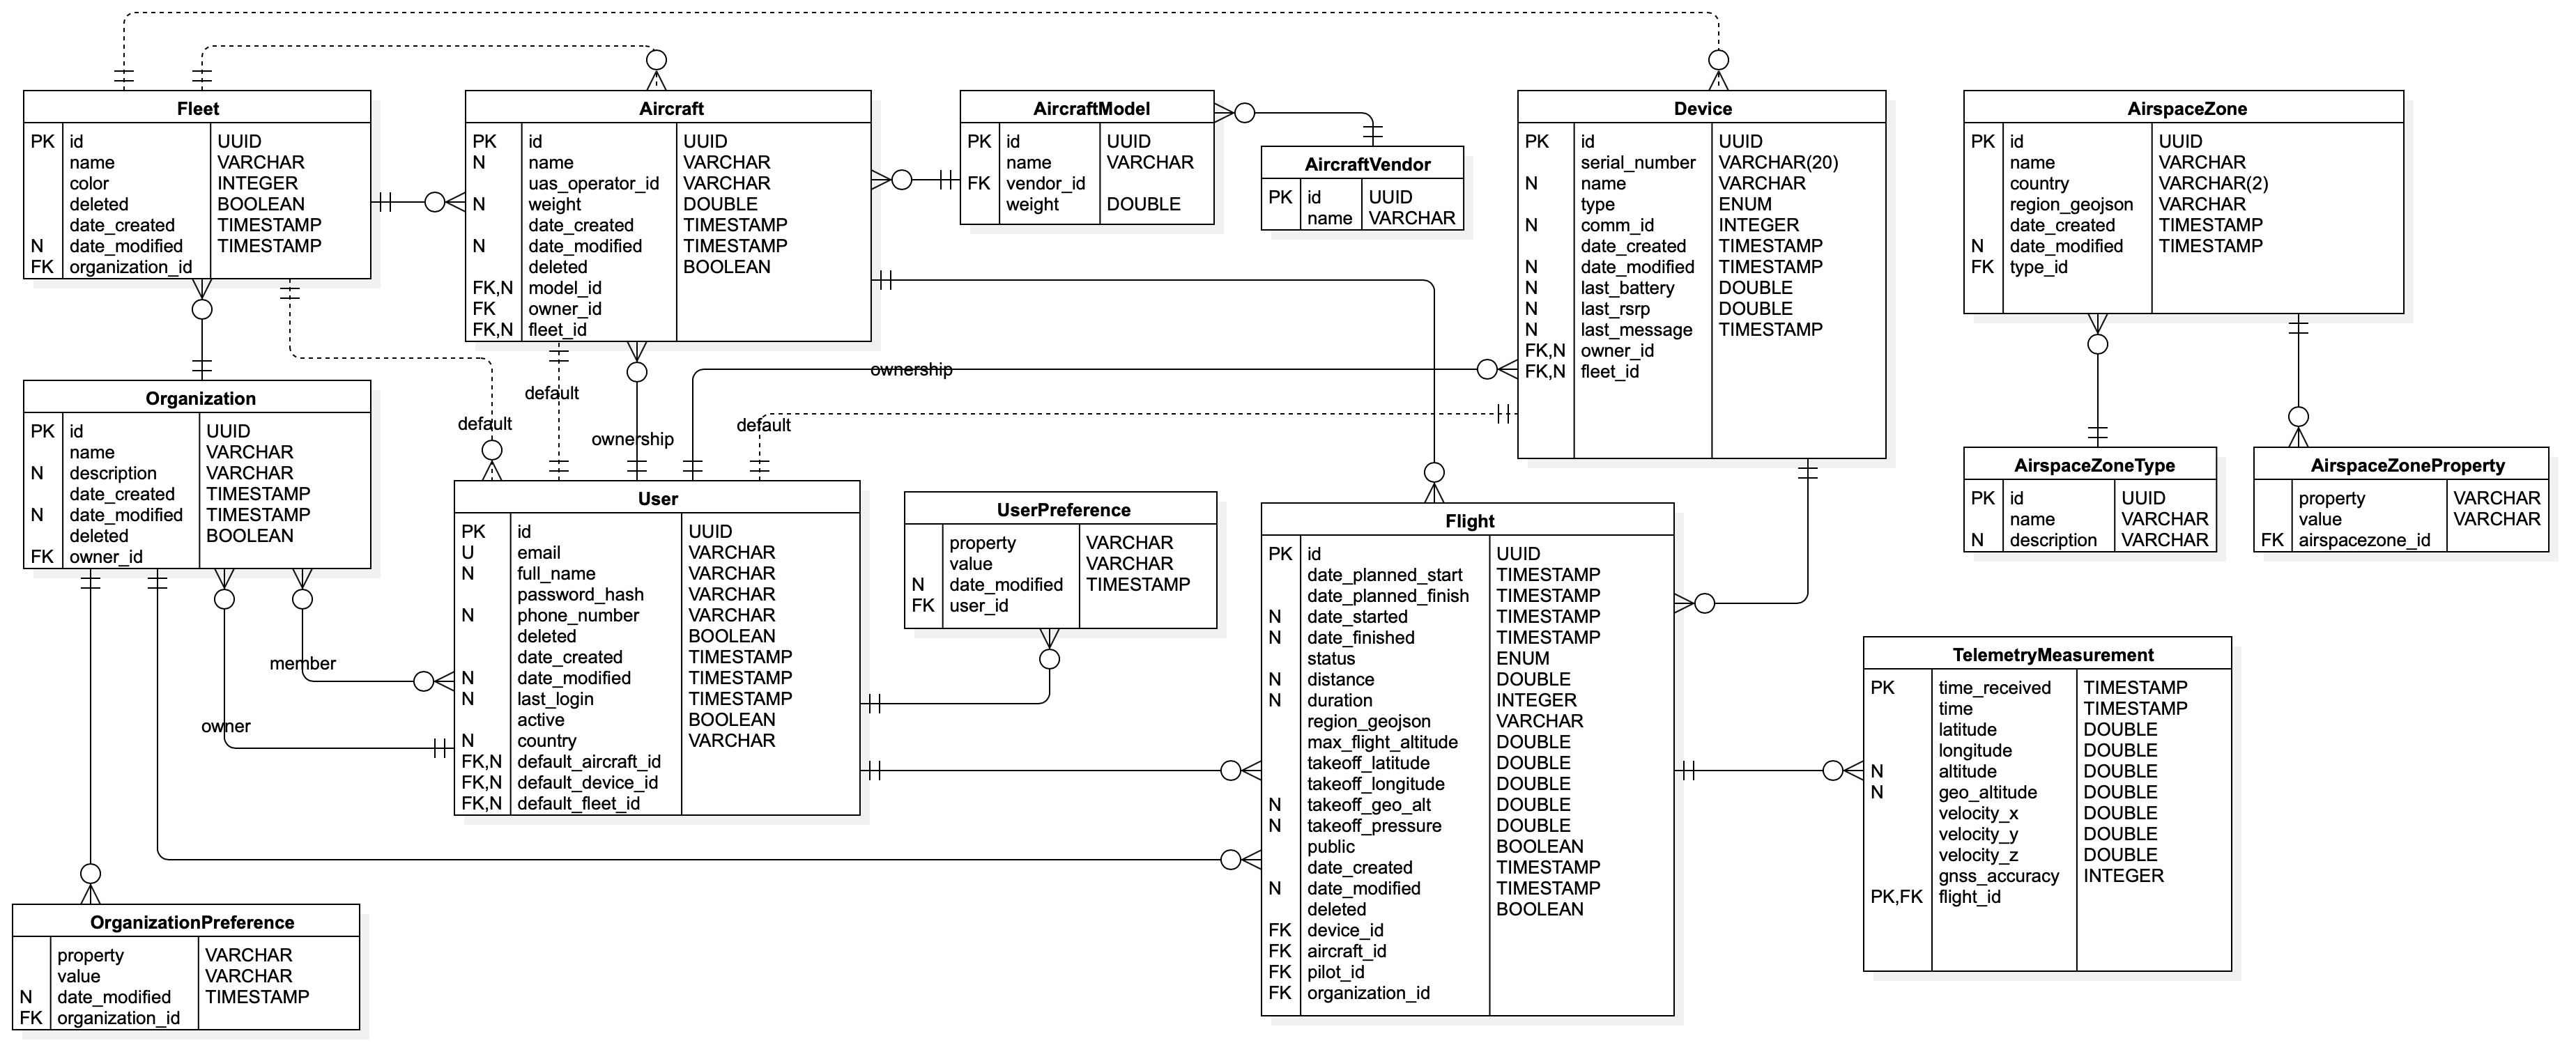
\includegraphics[scale=0.31, angle=90]{assets/erd_diagram.png}
    \caption{ERD Diagram of data model\cite{dataModel}}
    \label{fig:erd-diagram}
\end{figure}

\subsection{Live Service database model}\label{subsec:live-service-database-model}
In additional, during the development we had found out the current backend is not sufficient for our needs, so we decided to divide the backend model into backend one and Live Service model.
Because there are only live real time temporary data, so we deployed a Redis database.

"Redis is an open source (BSD licensed), in-memory data structure store, used as a database, cache and message broker.
It supports data structures such as strings, hashes, lists, sets, sorted sets with range queries, bitmaps, hyperloglogs, geospatial indexes with radius queries and streams.
Redis has built-in replication, Lua scripting, LRU eviction, transactions and different levels of on-disk persistence, and provides high availability via Redis Sentinel and automatic partitioning with Redis Cluster."\cite{redis}
It means that the Redis is a real-time storage that persists data only for very short time.
That is the reason, why it is suitable for this purpose.

The Live Service database model consists of \textbf{Device} and \textbf{Telemetry} entity.


%
%\begin{figure}
%    \centering
%    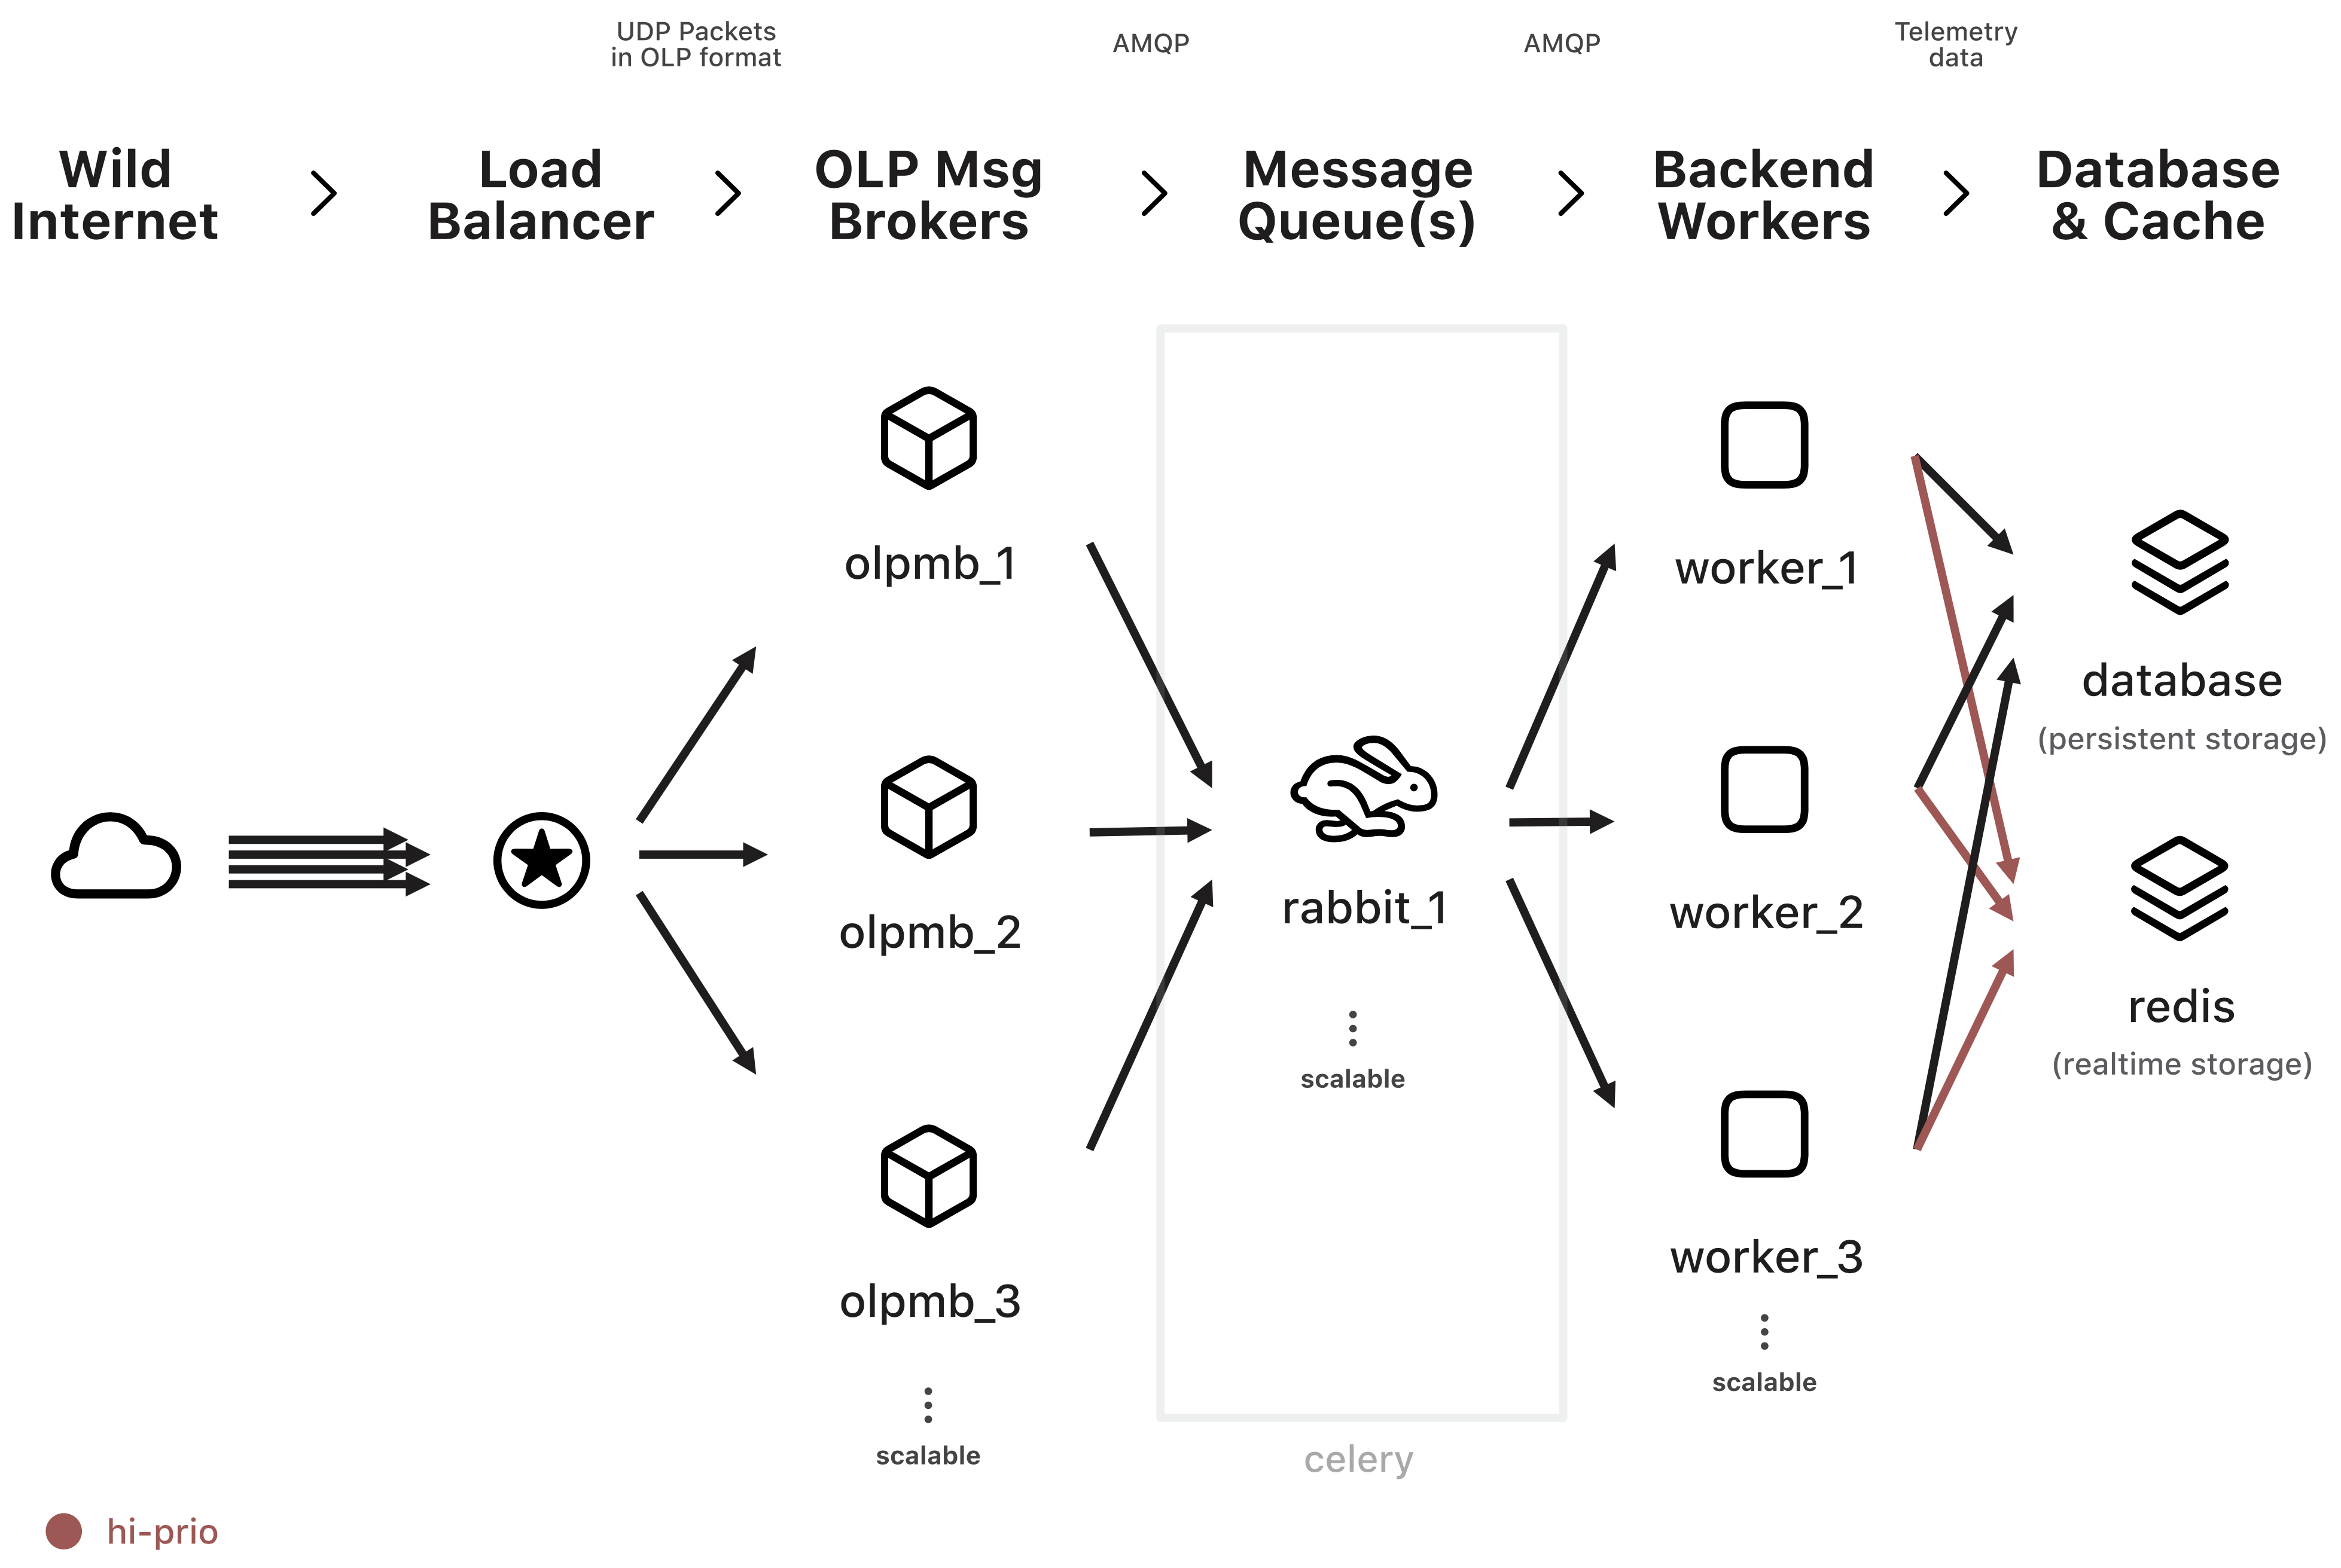
\includegraphics[scale=0.29, angle=90]{assets/infrastructure-diagram.png}
%    \caption{Infrastructure diagram~\cite{dataInfrastructure}}
%    \label{fig:infrastracture-diagram}
%\end{figure}

\chapter{Analysis of existing web and mobile applications}\label{ch:analysis-of-existing-web-and-mobile-applications}

TODO

\section{AirMap}\label{sec:airmap}
AirMap is the~main concurent application comparable with Dronetag platform.%\cite{}

\section{AisView}\label{sec:aisview}
TODO

\section{Fly carefully (L{\' e}tejte zodpov{\v e}dn{\v e})}\label{sec:fly-carefully}
TODO


TODO integration to foreign API endpoints


\chapter{Analysis of Flutter}\label{ch:analysis-of-flutter}

This chapter describes the key reasons why we chose Flutter for developing the mobile application.


\section{General concept}\label{sec:general-concept}
rendering widget similar to HTML

\subsection{Flutter UI}\label{subsec:flutter-ui}
Flutter has a widget tree that renders widget into nested tree and these widgets are covering themselves.

\section{Bloc}\label{sec:bloc}
Bloc is shortcut of Business Logic Component and allows separating your application into alone layers. It means that your application consists of following layer:
\begin{itemize}
    \item model - data model of your domain,
    \item UI - user graphical interface and 
    \item controller - it controls communication between data and UI layers.
\end{itemize}
Bloc represents the controller layer.
When your clicks on a button, it throws an event action that Bloc detects.
%\cite{bloc}

\subsection{HydratedBloc}\label{subsec:hydratedbloc}
HydratedBloc works as well as common Bloc.
The difference is in data storage.
Hydrated Bloc allow us to store data through a JSON object.
So, every time when your application loads data, you must not wait and show user progress indicator, but you are able to show stored data immediatelly.
And when you receive data, you will simply render it into screen.

\section{Widgets}\label{sec:widgets}
How the founder of Flutter say: ,,Everything in Flutter is Widget...".
It is true.
Each of components in Flutter UI is descendent of widget.
Many classes that inherit from a widget, but there are the essential descendants.
They are following:
\begin{itemize}
    \item StatelessWidget,
    \item StatefulWidget and
    \item InheritedWidget.
\end{itemize}{}
StatelessWidget is ... and offer ... \cite{statelessWidget}

StatefulWidget is ... and offer ... \cite{statefulWidget}

InheritedWidget is ... and offer reducing of boilerplate if you have many widgets nested in themselves.
Thanks the BuildContext class and of method, you can easily get the value you add as input variable.
... \cite{inheritedWidget}


\section{iOS specific UI widgets - Cupertino library}\label{sec:ios-specific-ui-widgets}
Cupertino is a library ...


\section{Android specific UI widgets - Material Design}\label{sec:android-specific-ui-widgets}
Material Design is a concept that was introduced by Google company ...

\chapter{User interface design}\label{ch:user-interface-design}

Describe a difference between Lo-Fi and Hi-Fi prototype.

I did not a Lo-Fi prototype because Dronetag is Start-up, company with limitted budget, so I focused only on the Hi-Fi. When I was making Hi-Fi, I inspired by a few concurrency application, which shows permitted flight zones and danger areas.
\section{Hi-Fi prototype}\label{sec:hi-fi-prototype}
I made a Hi-Fi prototype in Adobe XD.

\subsection{Dashboard}\label{subsec:dashboard2}

\subsection{Intro screen}\label{subsec:intro-screen}

\subsection{Login screen}\label{subsec:login-screen}

\section{Usability testing}\label{sec:usability-testing}
Describe usability testing flow

Describe right zoom when a user chooses drone on Dashboard map...

\subsection{Results}\label{subsec:results}

\subsection{Main mistakes in UI design}\label{subsec:main-mistakes-in-ui-design}
\chapter{Software architecture}\label{ch:software-architecture}
Describe software architecture - In Software development, Software architecture means the design of application from the higher perspective than Software design.
TODO
\section{Dependencies}\label{sec:dependencies}

\section{Bloc and Hydrated Bloc}\label{sec:bloc-and-hydrated-bloc}
In the begining, we counted on all of BLoCs will be the classic one.
After short time, we have found out the storable concept is more convenient for this purpose.
So, some of following are HydratedBloc...

\subsection{UserProfileBloc}\label{subsec:userprofilebloc}

\subsection{AircraftOperationBloc}\label{subsec:aircraftoperationbloc}

\subsection{DeviceOperationBloc}\label{subsec:deviceoperationbloc}


\section{JsonSerializable classes}\label{sec:jsonserializable-classes}

\section{Dio class}\label{sec:dio-class}

TODO
\chapter{Software design}
Describe software design

%-------------------------------------------------
\section{Common}
describe content
todo

%-------------------------------------------------
\section{IO}
todo

\subsection{Model}
Model is dedicated on objects that are produced by API endpoint of Dronetag backend.

\subsection{Respositories}
todo

\subsection{Services}
todo

%-------------------------------------------------
\section{UI}

\subsection{Aircrafts}
todo

\subsection{Common}
todo

\subsection{Dashboard}
todo

\subsection{Devices}
todo

\subsection{Flights}
todo

\subsection{Intro}
todo

\subsubsection{Login}
todo

\subsubsection{Registration}
todo

\subsection{Profile}
todo

%-------------------------------------------------
\section{Util}
todo

\subsection{Error}
todo

\subsection{Extensions}
todo

\subsection{Preferences}
todo

\chapter{Mobile application implementation}

Words about the implementation

\section{Build instructions}
TODO
\chapter{Code testing}\label{ch:code-testing}
TODO

\section{Unit testing}\label{sec:unit-testing}
TODO

\section{Integration testing}\label{sec:integration-testing}
TODO

\section{Mocker}\label{sec:mocker}
Mocker for flight drone simulations.
\chapter{Evaluation}
Evaluation about concept and encapsulation this app into Dronetag products.

\setsecnumdepth{part}
\chapter{Conclusion}\label{ch:conclusion}
% repeat problem statement
In this thesis, we talked about the problem of breaking laws by flight drones, and we also described zones type which the pilots have to avoid and flight levels.
Also, we clarified the differences among these zone types.

%related projects
We emphasized the analysis of related solutions for drone pilot support.
In this analysis, we described the key differences.

%backend infrastructure
In the backend infrastructure chapter, we introduced the all technology stack providing data, data model, and connection of these technologies.

%popsali jsme si basics of Flutter
We did not forget eighter on the Flutter basics and reasons why we chose the Flutter for cross-platform mobile application development and a brief comparison of the competition cross-platform frameworks.

%software architecture and design
We described the difference between Software architecture and design.
Then, we emphasized to the designed code structure of mobile application implementation.

%UI design
Further, it is still finding out that the UX/UI design has not been flawless initially.
This finding, we have revealed during the usability testing.
Hence, it is still improving, changing, and grouping the elements using the results from the first version of mobile application usability testing.

%deployment and testing
We described how to realize the implementation part of this thesis includes necessary steps to run the project in the development environment.
This description also contains the configuration files that must not check in with the version systems for security reasons.

We also talked about Software quality assurance and which methods we used in the mobile application.
We clarified the advantages and use cases of automation tests and chosen functions tested by Unit tests.

%evaluation
How we mentioned, one of the Dronetag products is the mobile application that will ensure safer drone operations.
This application is used as a client.
Thus it is directly dependent on the all platform, especially on the backend and Live service.
Hence, the development was divided into two main phases, called Alpha and Beta.

For the Alpha version release, we set the date to May 31st, 2020.
This version contains essential functionality like watching zones, drones, devices, and flight management, including searching and flight planning in two modes.
The first one is Fly now that allows a user to record his flight quickly.
The other is Plan a flight that allows a user to plan a flight on a specific time and place.
So, the Alpha version will provide the main application functionality.

In the next many months, we will be preparing the second version called Beta.
This version will emphasize performance optimization and use some data in an offline mode.
So, we want to ensure the full application functionality even in places with out-of-service.
Besides, it counts on the complete functionality realization of the fleet management for Organizations.
This functionality would be suitable for industrial purposes and ensure the safety of a bigger group of drones in the reserved area.
Most of the customers could be the companies doing business in the delivery of goods, watching around the airports, and medical systems to transfer medical materials to inaccessible places.
So, the Beta version will focus on the optimization and improvement of anything that will not have proven in the Alpha version.

%final conclusion
In conclusion, it is needed to emphasize the fact that the mobile application structure is still growing.
The fact gives it there are still implemented new and new functions that will contribute to more comprehensive using of the application.
In addition, there will need to be up-to-date with still more prominent use of drones in industry and still improving and adapting these technologies to the customers’ requirements.
Dronetag company reacts to these requirements a tries to offer a product that provides it and can be world-widely usable.




\bibliographystyle{template/iso690}
\bibliography{mybibliographyfile}

\setsecnumdepth{all}
\appendix

\chapter{Acronyms}\label{ch:acronyms}
% \printglossaries
\begin{description}
	\item[API] Application Interface
	\item[BLoC] Business Logic Component
	\item[CD] Continuous Delivery
	\item[CI] Continuous Integration
	\item[DI] Dependency Injection
	\item[GUI] Graphical user interface
	\item[Hi-Fi] High Fidelity
	\item[HTTP] Hypertext Transfer Protocol
	\item[IoC] Inversion of Control
	\item[JSON] Java Script Object Notation
	\item[Lo-Fi] Low Fidelity
	\item[POI] Point of Interest
	\item[SVG] Scalable Vector Graphics
	\item[UI] User Interface
	\item[URL] Uniform Resource Locator
	\item[UX] User Experience
	\item[XML] Extensible markup language
\end{description}


\chapter{SD card contents}\label{ch:sd-card-contents}

%change appropriately

\begin{figure}
	\dirtree{%
		.1 readme.txt\DTcomment{the file with SD card contents description}.
		.1 exe\DTcomment{the directory with executables}.
		.1 src\DTcomment{the directory of source codes}.
		.2 dronetag\DTcomment{implementation sources}.
		.2 thesis\DTcomment{the directory of \LaTeX{} source codes of the thesis}.
		.1 text\DTcomment{the thesis text directory}.
		.2 thesis.pdf\DTcomment{the thesis text in PDF format}.
	}\label{fig:figure}
\end{figure}

\end{document}


